\documentclass[12pt,halfline,a4paper,nonumbib]{ouparticle}

\usepackage[
backend=biber,
style=authoryear,
sorting=nyt,
citestyle=authoryear-comp,
maxcitenames=2,
maxbibnames=7
]{biblatex}

\addbibresource{references.bib}

%% My definition
\newcommand{\toshi}{\textcolor{blue}}


\usepackage{algorithm}
\usepackage{algorithmicx}
\usepackage{algpseudocode}

\begin{document}

\title{Is it me or my model talking? Validation of alternative model structures.}

\author{%
\name{Laurence T. Kell}
\address{ Centre for Environmental Policy, Imperial College London, Weeks Building, 16-18 Princes Gardens, London\\ SW7 1NE, UK}
\email{laurie@eaplusplus.co.uk}
\and
\name{Second Author}
\address{Institute or Organization, Department, City, State,\\
Zip Code, Country}
\email{e-mail address}
\and
\name{Toshihide Kitakado}
\address{Department of Marine Biosciences, Tokyo University of Marine Science and Technology, 4-5-7 Konan, Minato, Tokyo \\108-8477, Japan}
\email{e-mail address}
\and
\name{Fourth Author}
\address{Institute or Organization, Department, City, State,\\
Zip Code, Country}
\email{e-mail address}
\and
\name{Fifth Author}
\address{Institute or Organization, Department, City, State,\\
Zip Code, Country}
\email{e-mail address}
\and
\name{Max Cardinale}
\address{Swedish University of Agricultural Sciences, Department of Aquatic Resources, Institute of Marine Research, Lysekil,\\ Sweden}
\email{massimiliano.cardinale@slu.se}}

\abstract{
}

\date{\today}

\keywords{cross-validation, diagnostics, hindcast, retrospective analysis, stock assessment, validation}

\maketitle

\section{Introduction}

Stock assessment models are a key element of fisheries management, however, there are various definitions of stock assessment \parencite[e.g.][]{hilborn2003state,cadrin2014stock}. We prefer "The description of the characteristics of a 'stock' so that its biological reaction to being exploited can be rationally predicted and the predictions tested" (Holt pers comm.). The reason for our preference is because this explicitly recognises that the main aim of a stock assessment is to provide the basis for the long-term sustainable management of fisheries resources. This requires making and validating probabilistic estimates of stock status and forecasts of the consequences of management actions.

Model validation is important in many fields, e.g. in energy and climate modelling \parencite{kell2019optimising}, as this increases confidence in the outputs of a model and leads to an increase in trust amongst the public, stake and asset-holders and policy makers \parencite[][]{saltelli2020five}. Therefore, after a model structure has been agreed and parameters estimated, it is crucial to validate the model. Validation assesses whether it is plausible that the data were generated by a system identical to the model \parencite{thygesen2017validation}. The ambition of validation is not to prove that a model is correct, but to check that the model cannot be falsified with the available data. This is different question from asking is the model fit for a given purpose, which depends on the objectives for which the model was developed. For example to evaluate whether an assessment model help achieve maximum sustainable yield requires conducting Management Strategy Evaluation \parencite[MSE,][]{punt2007developing}; see \cite{sharma2020trfmo} for a review of current practice in the tuna Regional Fisheries Management Organisations (tRFMOs).   

Model validation serves a purpose complementary to model selection and hypothesis testing. Model selection searches for the most suitable model within a specified family, hypothesis testing examines if the model structure can be reduced, and model validation examines if the model family should be modified or extended. For models to be valid they must satisfy four prerequisites \parencite{hodges1992you}: the situation being modelled must (i) be observable and measurable, (ii) it must be possible to collect sufficient data informative about it, (iii) exhibit constancy of structure in time, and (iv) exhibit constancy across variations in conditions not specified in the model. The first two prerequisites should be straight forward, however, many stock assessments (e.g. for highly migratory stocks fished in areas beyond national jurisdiction), rely on fisheries dependent data rather than direct scientific observations. This is of concern since \cite{harley2001catch} found strong evidence that commercial catch per unit effort (CPUE) was likely to remain high while abundance declines.  Prerequisite (iii) ensures that the model has prediction skill for the same conditions under which the validation tests were conducted, while prerequisite (iv) ensures that the model will still be valid for conditions that differ from those in the validation tests, i.e. can be used to set robust management advice.

A common tool in stock assessment is retrospective analysis to check the stability of past model estimates\parencite{hurtado2014looking}. In a retrospective analysis data from the most recent years are sequentially removed and the model refitted and estimates of spawning stock biomass (SSB) and fishing mortality compared. Stability of historical estimates, however, can be achieved at the expense of the accuracy and precision of forecasts. We therefore extend retrospective analysis by projecting forward for the reported catch over the years removed. 

The use of model based quantities, however, is not sufficient to fulfill prerequisite i). We therefore, conduct model-free hindcasts to estimate prediction skill by comparing observations of indices of relative abundance to model estimates of the same quantities (pseudo observations). Prediction skill is a statistical measure of the accuracy of a forecast compared to an observation or estimate of the actual value of what is being predicted \parencite{huschke1959glossary}, and can be used to compare alternative models or observations to a reference set of estimates or data \parencite{jin2008current, weigel2008can, balmaseda1995decadal}.
 
We compare three model structures used in the assessment of Indian Ocean yellowfin tuna stock, namely a full integrated model (SS3), an age structured production model (ASPM), and a biomass dynamic model (JABBA). We do this by first using model-based quantities and then using peudo observations to estimate prediction skill. The use of prediction skill allows the different model structures and data components to be compared in order to identify potential model mis-specification and data conflicts. 

%We discuss hypothesis testing, model selection and model validation, then make recommendations for the bench-marking of stock assessment methods.

\section{Material and Methods}
Indices of abundance are a key contributor to the overall likelihood when fitting stock assessment models to data \parencite{whitten2013accounting}, and the sum of squared errors (SSE) between observed and predicted indices in log-space is the measure of fitness. When comparing models, however, the SSE is problematic because complex models tend to have many parameters to allow flexibility when fitting, which may result in a low SSE due to overfitting. Therefore, information criteria, such as AIC, have been developed to aid in model selection. AIC is only a relative measure of the appropriateness of models, however, and additional diagnostic tests are required for model validation. This is of particular importance for stock assessment models where only a single historical data set exists, and the system can not be observed directly. 

The objective of this study therefore is to devlop a procedure to validate and compare different families of models based on past events. To do this we extend retrospective analysis to conduct model-based and model-free hindcasts, by adding the additional step of projecting over the truncated years. Comparing model outputs with observations allows prediction skill to be estimated \parencite{kell2016xval}, defined as any measure of the accuracy of a forecasted value compared to the actual (i.e. observed) value that is not known by the model \parencite{glickman2000glossary}. 

\subsection{Materials}

For our example we use the stock assessment of yellowfin tuna (\textit{Thunnus albacares}) conducted by the Indian Ocean Tuna Commission \parencite{IOTWPTT21}. Yellowfin tuna supports one of the largest tuna fisheries in the Indian Ocean, with catches currently exceeding 400,000t. They are harvested by a variety of gears, from small-scale artisanal fisheries, to large gillnetters, and industrial longliners and purse seiners \parencite{fiorellato2019tt}.

The main assessment is conducted using Stock Synthesis \parencite[SS,][]{methot2013stock}, although other methods are also employed. SS implements an age and spatially structured model that reflects the complex population and fishery dynamics of the stock. Model development has focused on spatial structure to account for the differences in regional exploitation patterns, incorporating seasonal movement dynamics, resolving data conflicts, and exploring non-stationary in selectivity and catchability \parencite{urtizberea2018yft}. The data used includes time series of total catch and four CPUE indices based on the long-line fisheries, spatially stratified in four regions (figure \ref{fig:map})
 
The most recent assessment established a base case as a reference model for diagnostics along with scenarios to capture a range of uncertainties \parencite{fu2018yft}. The assessment indicates that the stock  has declined substantially since 2012, and spawning stock biomass in 2017 is now estimated to be close to the historical lowest level. The stock is estimated to be overfished, and so the IOTC has implemented a rebuilding plan to reduce overall fishing pressure.  

The base case is spatially disaggregated into two tropical regions that encompass the main year-round fisheries and two austral, subtropical regions where the long-line fisheries occur more seasonally \parencite{langley2015yft}, with reciprocal movement assumed to occur between adjacent regions. The SS assessment is based on a quarterly time step to approximate the continuous recruitment and rapid growth seen in the stock. Twenty-five fisheries were defined based on fishing gear, region, time period, fishing mode and vessel type. Most fisheries were modelled allowing flexibility in selectivity (e.g. cubic spline or double normal), whereas long-line selectivity was constrained to be fully selective for the older ages. The population comprised 28 quarterly age-classes with an assumed unexploited equilibrium initial state in each region. 

Recruitment occurs in the two equatorial regions with temporal deviates in the regional distribution and was assumed to follow a Beverton and Holt stock recruitment relationship (with a steepness of 0.8 and recruitment standard deviation of 0.6).  Growth was parameterised using age-specific deviates on the $k$ growth parameter to mimic the non-von Bertalanffy growth of juvenile and the near linear growth of adults. Natural mortality is variable with age, with the relative trend in age-specific natural mortality based on the values applied in the Pacific Ocean \parencite{maunder2012review}. 

%[Maunder, M.N., Aires-da-Silva, A. 2012. A review and evaluation of natural mortality for the assessment and management of yellowfin tuna in the eastern Pacific Ocean. External review of IATTC yellowfin tuna assessment. La Jolla, California. 15-19 October 2012. Document YFT-01-07.]

The data used for fitting are catch and length composition data, long-line CPUE indices, tagging recaptures, and environmental data. The length composition was weighted such that they were sufficient to provide reasonable estimates of fishery selectivity and recruitment trends but not directly influence the trends in stock abundance. Regional environmental indices (current and sea temperature) allows seasonal and temporal variations to be incorporated in the estimation of fish movement. 

The CPUE indices represent the primary source of information on abundance and is based on a composite long-line index from the main distant water fleets %\parencite{hoyle2018yft}. 
Indices in each region were standardised using generalised linear models that accounted for differences in targeting practices and catchability amongst fleets, based on gear configurations and species composition. The reason for this is because tuna long-line fishing strategies have changed over time %\parencite{hampton2005}. 
In the assessment, the CPUE indices across regions were linked by a common catchability coefficient, thus improving the ability of the model to estimate the distribution of biomass by region. %\parencite{langley2015yft, fu2018yft}.

Tag release/recovery data collected from the main phase of the Indian Ocean large-scale tuna tagging programme %[Hallier 2008] 
were integrated into the model to inform estimates of fishing mortality, abundance, and movement. 

%[Hallier 2008. STATUS OF THE INDIAN OCEAN TUNA TAGGING PROGRAMME - RTTP-IO. IOTC-2008-WPTDA-10]

\subsection{Assessment Methods}

There has been a recent trend in stock assessment toward the use of integrated analysis that combines several sources of data into a single model by a joint likelihood for the observed data \parencite[e.g.][]{doubleday1976least,fournier1982general,maunder2013review}. Datasets include records of catches and landings, indices of abundance based on catch per unit (CPUE) or from research surveys, and length and age compositions based on samples. An example of commonly used integrated assessment method is SS3 that can be configured in multiple ways, allowing for a range of scenarios to be developed to reflect uncertainty.

For example \cite{maunder2015contemporary} proposed a deterministic implementation of an age-structured production model (ASPM) as a diagnostic of process dynamics. Selectivity in ASPM is parameterised based on the selectivity estimated by a "full" SS model. The model is then fitted to the abundance indices, assuming a deterministic spawning recruitment relationship, and without the size composition data contributing to the likelihood function. This enables an evaluation of whether the observed catches alone can explain trends in the index of abundance. If the ASPM is able to fit the indices of abundance well then a production function is likely to exist (i.e. the dynamics are driven by density dependent processes), and the indices provide information about absolute abundance. If  the fit is poor, then the catch data alone cannot explain the trends in the indices. This can have several causes, namely (i) stock dynamics are recruitment-driven, (ii) the stock has not yet declined to the point at which catch is a major factor influencing abundance; (iii) the indices of relative abundance are not proportional to abundance;  (iv) the model is incorrectly specified; or (v) the data are incorrect

The ASPM has been shown \parencite{carvalho2017can} to be the best method for detecting misspecification of the key systems-modeled processes that control the shape of the production function. This is a problem since many of the required parameters in integrated assessments are difficult to estimate \parencite[e.g.][]{lee2011m,lee2012steepness} and have to be fixed or priors used. 

An alternative to an integrated assessment is to use a biomass dynamic model, based on an explicit production function, that requires the estimation and fixing of fewer parameters. An example is JABBA, an open source package that presents a unifying, flexible framework for biomass dynamic modelling, runs quickly, and generates reproducible stock status estimates \parencite{winker2018jabba}.The model uses a Pella Tomlinson production function that allows the shape of the production function to be varied, and alternative assumptions about productivity, stock status and reference points to be evaluated. 

The base case SS assessment conducted by the Indian Ocean Tuna Commission (IOTC) for Yellowfin Tuna, was reconfigured as an ASPM and as a biomass dynamic assessment. In the later case in order to mimic the dynamics of the base case assessment, the production function parameters were tuned to the base case Stock synthesis assessment. 

\subsection{Hindcast}

Retrospective analysis \parencite{hurtado2014looking} is commonly used to evaluate the stability of stock assessment estimates from alternative models. Observations are sequentially removed from the terminal year, the model is then refitted to the truncated series and the difference between between estimates from the full and truncated time-series compared using the relative error (RE, a measure of bias). 

Hindcasting like traditional retrospective analysis involves fitting a model using a tailcutting procedure, where data are deleted sequentially for $n$ years, i.e. from the last year $T$ through to $T−n$, the additional step in the hindcast is that then the data from year 1 to $T - n - 1$ are used to make predictions of what will happen in years $T - n$ to $T$.

Since assessment cycles are typically for three years  with advice \parencite{fricker2013three} we projected the truncated estimates for 3 years. We chose 3 years as that is essentially the time-step between assessments in most tuna Regional Fisheries Management Organisations.

\begin{algorithm}[!ht]
\begin{algorithmic}[1]
\State Fit model up to and including terminal year $T$
\For{$t$ = $T - 3$ to n} 
\State fit model to data up to time $t$ \For {$i$ = $t$ to $t + 3$} 
\State Estimate $\hat{y_i}$
\EndFor
\EndFor
\caption{Hindcast}
\label{Hindcast}
\end{algorithmic}
\end{algorithm}

When conducting the hindcast it is assumed that modelled variables are observable, processes exhibit constancy of structure in time, including those not specified in the model, and that collection of accurate and sufficient data is possible \parencite{hodges1992you}.

\subsubsection{Prediction Skill}


The use of model based quantities means that bias can not actually be quantified. For example a reduction in both relative error (a measure of bias) and mean squared error (a measure of variance) can be achieved by shrinking terminal estimates towards recent historical values, at the expense of prediction skill. The absence of retrospective patterns in model based quantities, therefore, while reassuring is not sufficient for model validation, and model-free validation using prediction residuals should be used as well.

Inspection of residuals is a common way to determine a model’s goodness-of-fit \parencite{cox1968general}, since  non-random patterns in the residuals may indicate model misspecification, serial correlation in sampling/observation error, or heteroscedasticity. When inspecting residuals, however, there is a danger of hypothesis fishing/testing?, i.e. [I read the sentence below a few times but could not make sense of it probably need revising?] choosing a scenario retrospectively retrospect, while if multiple true hypotheses are tested it is likely that some of them will be rejected. Therefore it is valuable to reserve part of the data to test for validation, so that a pattern’s significance is not tested on the same data set which suggested the pattern \parencite{thygesen2017validation}. For this reason we conduct a model-free hindcast to estimate prediction skill.

\subsubsection{Metrics}

For the evaluation of model-based quantities, we use Mohn's rho ($\rho_M$ \toshi{$\rho_{Mr}$?}, equation \ref{eqn:mohn}) and a modified version ($\rho_{Mr}$ \toshi{$\rho_{p}$?}, equation \ref{eqn:mohn2}). \toshi{IF my understanding above on $\rho_{p}$ is correct, this is also for assessing prediction skill but "model based". I think we can highlight here difference in model-based and model-free in addition to model validation with/without prediction.}

We used the mean absolute scaled error (MASE, equation \ref{eqn:mase}) to evaluate prediction skill. The best statistical measure to use depends, however, on the objectives of the analysis and using more than one measure can be helpful in providing insight into the nature of observation and process error structures \parencite{kell2016xval}. Therefore we also use root mean squared error ($E^{\prime 2}$, equation \ref{eqn:rmse}), correlation ($\rho$) and the standard deviation ($\sigma$). 

$E^\prime$ is a commonly used metric, as the square root of a variance it can also be interpreted as the standard deviation of the unexplained variance,  lower values indicate better fits. $E^\prime$ is sensitive to outliers, however,and favours forecasts that avoid large deviations from the mean and cannot be used to compare across series. The correlation ($\rho$) in contrast is unaffected by the amplitude of the variations, insensitive to biases and errors in variance, and can be used to compare across series. $E^{\prime 2}$ and $\rho$ are related by the cosine rule i.e.

 \begin{equation} 
 E^{\prime 2} = \sigma_o^2 + \sigma_f^2 - 2\sigma_o\sigma_f\rho
 \end{equation}

Where the reference set ($o$) are the observations not included in the retrospective assessment and the values ($f$) are their estimates. 
 
This means that $E^\prime$, $\rho$ and $\sigma_f$ can be summarised simultaneously in a single diagram\parencite{taylor2001summarizing} providing a concise statistical summary of how well patterns match each other and are therefore especially useful for evaluating multiple aspects or in gauging the relative skill of different models \parencite{griggs2002climate}.

\section{Discussion}

\begin{itemize}
 \item The description of the characteristics of a 'stock' so that its biological reaction to being exploited can be rationally predicted and the predictions tested"
 \item Hypotheses about states of nature are represented by alternative model structures and fixed parameters, e.g. grids, howewver, the choice of scenarios is often arbitrary, there is no weighting or rejection, and the grid stops model development. 
 \item Need for validation; for which prerequisites are
 \begin{itemize}
  \item (i) observable and measurable, 
  \item (ii) possible to collect sufficient data informative about it, 
  \item (iii) exhibit constancy of structure in time, and 
  \item (iv) exhibit constancy across variations in conditions not specified in the model. 
 \end{itemize}
  \item The accuracy and precision of the predictions depend on the validity of the model, the information in the data, and how far ahead we wish to predict (i.e. the prediction horizon). 
  \item If a model is not validated then it may not be possible to use it for prediction, but that depends on the purpose 
  \item There are still uses, however, for non predictive models, e.g. for scenario modelling or as part of a feedback management system. 
  \item How to agree the scenarios to include and the weighting and acceptance criteria. Weighting of grids based on AIC and likelihoods is only really possible if you use a common modelling framework like SS. In most if not all cases, however, the problems are unknown parameter values and data weighting. In which case the best approach is to develop robust management procedures. There is a need therefore to develop OMs based on hypotheses we can resolve, i.e. show the value of information. In the mean time we need to develop robust MPs based on the value of control.
  \item The factors that impact on HCRs are trends and fluctuations in populations are determined by complex interactions between extrinsic forcing and intrinsic dynamics. For example, stochastic recruitment can induce low-frequency variability, i.e. ‘cohort resonance’, which can induce apparent trends in abundance and may be common in age-structured populations \parencite{bjoernstad2004trends, botsford2014cohort}. Such low-frequency fluctuations can potentially mimic or cloak critical variation in abundance linked to environmental change, over-exploitation or other types of anthropogenic forcing. 

\end{itemize}

\section{Conclusions}

\newpage
\printbibliography

\section{Tables}

\begin{table}[!ht]
\caption{Mohn's ($\rho_{Mr}$) for retrospective analysis.}  
\begin{center}
\label{tab:retro-rho}
\begin{tabular}{|cccc|}
\hline
	\tiny Method	& {\tiny Quantity}  & {\tiny Retrospective} & {\tiny Projection} \\ 
\hline\hline
{\tiny SSB          } & {\tiny SS} 	     & {\tiny    0.04} & {\tiny  0.32}      \\
{\tiny SSB          } & {\tiny ASPM} 	 & {\tiny   -0.03} & {\tiny -0.09}      \\
{\tiny SSB          } & {\tiny JABBA} 	 & {\tiny   -0.09} & {\tiny -0.21}      \\
{\tiny F            } & {\tiny SS} 	     & {\tiny   -0.15} & {\tiny -0.24}      \\
{\tiny F            } & {\tiny ASPM} 	 & {\tiny    0.03} & {\tiny  0.08}      \\
{\tiny Harvest Rate } & {\tiny JABBA} 	 & {\tiny   -0.09} & {\tiny -0.09}      \\
\hline
\end{tabular}
\end{center}
\end{table}

\begin{table}[ht]
\caption{Model-free results}
\centering
\label{tab:mase}
\tiny
\begin{tabular}{|cc|ccc|ccc|ccc|ccc|}
  \hline
 CPUE & Quarter &  & MASE &  &  & RMSE & &  & $\rho$ &  & & $\sigma$ &  \\
      &         & SS & ASPM & JABBA & SS & ASPM & JABBA & SS & ASPM & JABBA & SS & ASPM & JABBA \\
\hline\hline
  1 & 1 & 1.04 & 0.56 & 0.98 & 0.46 & 0.26 & 0.42 & 0.45 & 0.74 & 0.34 & 0.45 & 0.27 & 0.41 \\ 
  1 & 2 & 0.80 & 0.44 & 0.95 & 0.34 & 0.20 & 0.38 & 0.69 & 0.90 & 0.44 & 0.34 & 0.21 & 0.39 \\ 
  1 & 3 & 1.33 & 0.99 & 1.08 & 0.50 & 0.39 & 0.35 & 0.48 & 0.32 & 0.47 & 0.42 & 0.38 & 0.30 \\ 
  1 & 4 & 1.13 & 0.58 & 1.23 & 0.39 & 0.23 & 0.36 & 0.51 & 0.69 & 0.46 & 0.40 & 0.23 & 0.33 \\ 
  2 & 1 & 1.91 & 1.48 & 1.51 & 0.46 & 0.34 & 0.42 & 0.18 & 0.70 & 0.29 & 0.43 & 0.21 & 0.29 \\ 
  2 & 2 & 2.29 & 1.83 & 2.03 & 0.74 & 0.59 & 0.59 & -0.33 & 0.14 & 0.06 & 0.57 & 0.36 & 0.32 \\ 
  2 & 3 & 1.50 & 1.10 & 1.05 & 0.46 & 0.32 & 0.30 & 0.33 & 0.34 & 0.16 & 0.44 & 0.28 & 0.25 \\ 
  2 & 4 & 1.60 & 1.97 & 1.63 & 0.50 & 0.49 & 0.40 & 0.44 & 0.61 & 0.30 & 0.39 & 0.24 & 0.26 \\ 
  3 & 1 & 1.65 & 0.71 & 0.68 & 0.52 & 0.22 & 0.23 & 0.27 & 0.73 & 0.66 & 0.40 & 0.22 & 0.24 \\ 
  3 & 2 & 1.43 & 0.96 & 1.36 & 0.46 & 0.31 & 0.36 & 0.42 & 0.63 & 0.82 & 0.41 & 0.31 & 0.19 \\ 
  3 & 3 & 1.53 & 0.86 & 1.34 & 0.38 & 0.26 & 0.31 & 0.49 & 0.64 & 0.76 & 0.35 & 0.24 & 0.20 \\ 
  3 & 4 & 1.03 & 0.75 & 1.07 & 0.52 & 0.34 & 0.41 & 0.70 & 0.84 & 0.86 & 0.39 & 0.33 & 0.42 \\ 
  4 & 1 & 4.02 & 0.96 & 2.99 & 0.75 & 0.21 & 0.48 & 0.47 & 0.84 & 0.90 & 0.44 & 0.22 & 0.16 \\ 
  4 & 2 & 1.74 & 0.66 & 1.28 & 0.82 & 0.34 & 0.47 & 0.50 & 0.81 & 0.78 & 0.56 & 0.35 & 0.37 \\ 
  4 & 3 & 3.45 & 1.04 & 2.13 & 0.86 & 0.27 & 0.49 & 0.33 & 0.69 & 0.73 & 0.55 & 0.28 & 0.21 \\ 
  4 & 4 & 5.79 & 1.28 & 5.12 & 0.82 & 0.20 & 0.51 & 0.50 & 0.88 & 0.90 & 0.53 & 0.18 & 0.15 \\ 
 \hline
\end{tabular}
\end{table}

\section{Figures}

\begin{figure*}[!ht]
\centering
\includegraphics[width=6in]{figures/map.png}
\caption{Spatial stratification of the Indian Ocean for the four region assessment model (R1a and R1b were treated as one model region but were retained for the fleet definition). The black arrows represent the configuration of the movement parameterization.  Density contours represent of the dispersal of tag releases (red) and subsequent recaptures from Indian Ocean Regional tuna tagging programme. Green circles represent the distribution of catches from the longline fishery aggregated by 5 degree longitude and latitude for 1980 to 2017 (max. = 133 770 t).}
\label{fig:map}
\end{figure*}


\begin{figure*}[!ht]
\centering
\includegraphics[width=6in]{figures/ll.png}
\caption{Regional longline CPUE indices included in the 2018 stock assessment. The difference in scales represents the relative distribtuion of longline vulnearable biomass amongst regions.}
\label{fig:ll}
\end{figure*}

\begin{figure*}[htbp]
\centering
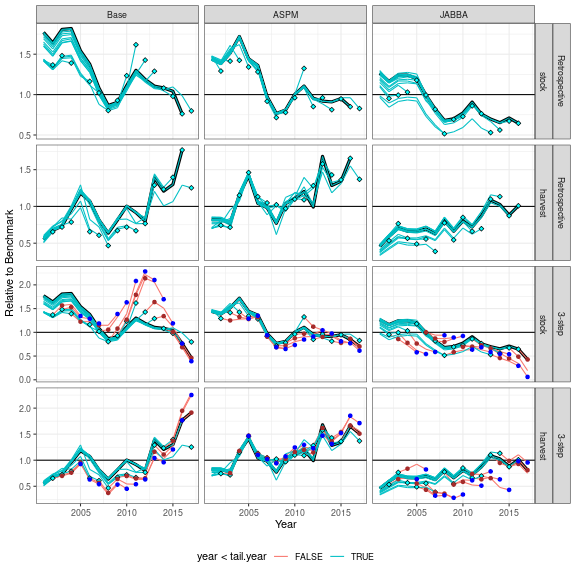
\includegraphics[width=6in]{figures/final-retro-all-1.png}
\caption{Retrospective analysis for the three models, points indicate the terminal years, and the think line the assessment using all the data.}
\label{fig:retro}
\end{figure*}

\begin{figure*}[htbp]
\centering
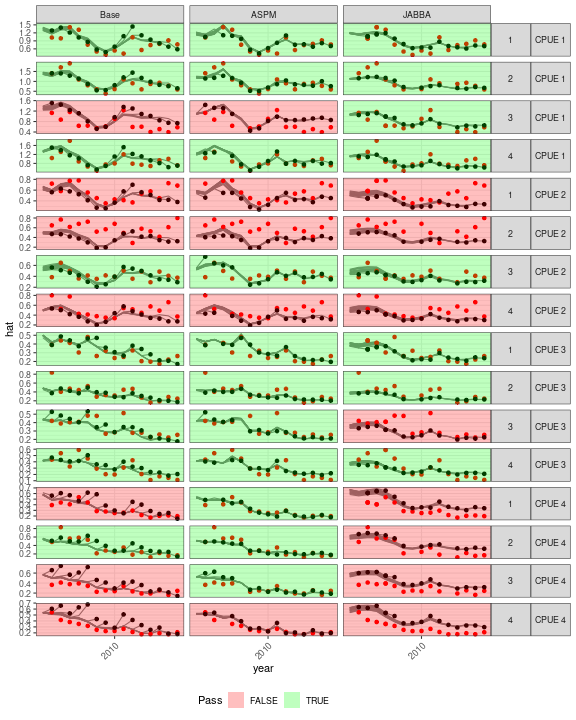
\includegraphics[width=6in]{figures/final-hy-plot-1.png}
\caption{Hindcasts for one step ahead predictions, red dots are the observed CPUE values and lines are the fits with terminal hincast year indicated by a point.}
\label{fig:hy}
\end{figure*}

\begin{figure*}[htbp]
\centering
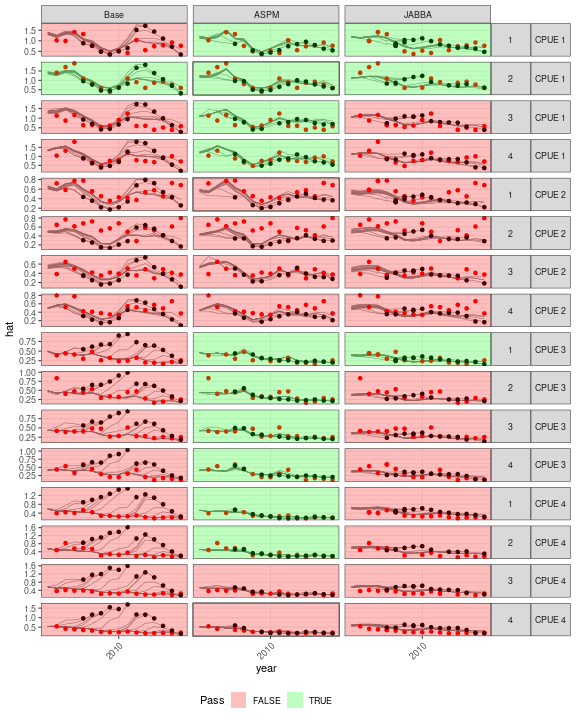
\includegraphics[width=6in]{figures/final-hy3-plot-1.png}
\caption{Hindcasts for three step ahead predictions, red dots are the observed CPUE values and lines are the fits with terminal hincast year indicated by a point.}
\label{fig:hy3}
\end{figure*}

\begin{figure*}[htbp]
\centering
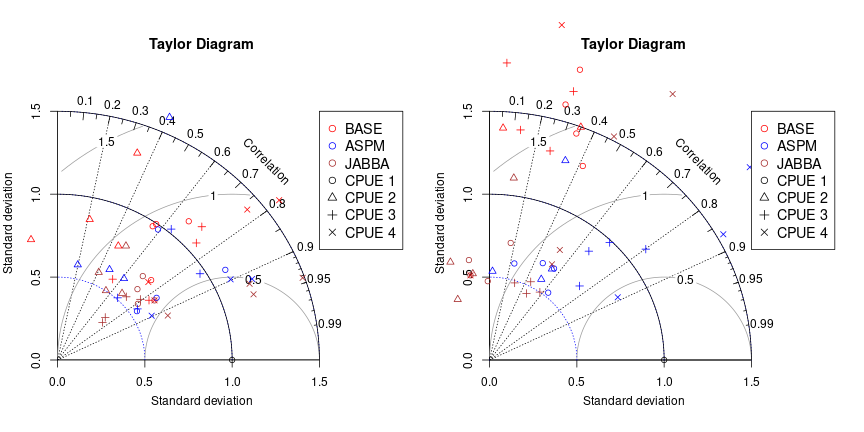
\includegraphics[width=6in]{figures/final-taylor-hy-1-1.png}
\caption{Taylor diagram for one and three year ahead predictions,  summarising the similarity between the observed time series of CPUEs and the predicted relative stock abundance. Each point quantifies how closely predictions match observations, the angle indicates the correlation, the centred root-mean-square error difference between the predicted and observed patterns is proportional to the distance to the point on the x and the contours around this point indicate the RMSE values; the standard deviations of the predictions are proportional to the radial distance from the origin, scaled so the observed pattern has a value of 1. The open circle corresponds to a series which is identical to the reference series. The colours correspond to the model and shape to the survey.)}
\label{fig:td}
\end{figure*}

\begin{figure*}[htbp]
\centering
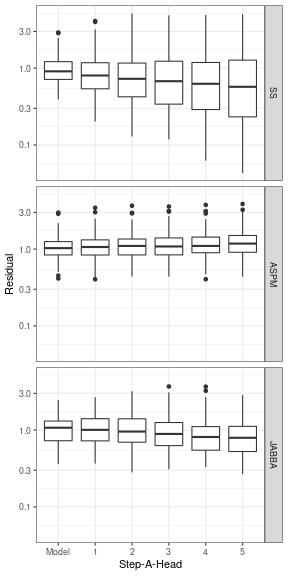
\includegraphics[width=4in]{figures/final-rsdl-1.png}
\caption{Residual for model (Step 0) and predictiion residuals for 1,2,3,4 and 5 steps ahead.}
\label{fig:residuals}
\end{figure*}

\subsection{Appendix}
\label{metrics}

\appendix* 
\subsection{Metrics}

Indices of abundance are a key contributor to the overall likelihood when fitting stock assessment models to data. The Sum of Squared Errors (SSE) between observed and predicted indices in log-space is the measure of fitness. When comparing models, however, the SSE is problematic because complex models tend to have many parameters to allow flexibility when fitting, which may result in a low SSE due to overfitting. Therefore, information criteria, such as AIC, have been developed to aid in model selection. AIC is only a relative measure of the appropriateness of models, and additional diagnostic tests are required for model validation. This is of particular importance for stock assessment models where only a single historical data set exists, and the system can not be observed directly.

Therefore in stock assessment, a standard diagnostic is to evaluate retrospective bias as proposed by \cite{mohn1999retrospectyive}. As described in earlier sections, the retrospective analysis can be conducted by sequentially refitting the model to reduced data sets by removing some recent years' data to see if there are any systematic pattern within a model. The retrospective bias is then evaluated using the so-called Mohn's rho as 

\begin{equation}
\label{eqn:mohn0}
\rho_M = \disp \sum_{t=T-n}^{T-1} \frac{\hat{y}_{(1:t),t}-\hat{y}_{(1:T),t}}{\hat{y}_{(1:T),t}}, 
\end{equation}

where $\hat{y}$ denotes in general a value like estimated biomass, 1+population size, or predicted abundance index, and the value with suffix $\hat{y}_{(1:t^\prime),t}$ means such a value estimated at time $t$ of a full series from 1 to $T$ using a retrospective data window from 1 to $t^\prime (\leq T)$. In this paper, we will use a variant of the original $\rho$ as the mean (average) like 
\begin{equation}
\label{eqn:mohn}
\rho_{Mr} = \disp \frac{1}{n} \sum_{t=T-n}^{T-1} \frac{\hat{y}_{(1:t),t}-\hat{y}_{(1:T),t}}{\hat{y}_{(1:T),t}} 
\quad \mbox{[rho for retro-bias]}, 
\end{equation}
This metric is an average of relative differences at the final time of each window. Therefore it is a measure of relative retrospective `bias' (scale-free) in a statistical sense. The metric tends to be applied not on the log but the original scale because both the directions of positive and negative biases are regarded as being equivalent. 

Hindcasting, which is the primary focus in this paper is a form of retrospective cross-validation, and therefore an extension of retrospective analysis which projects several steps forward beyond the retrospective data window to quantify the prediction skill of a model. Theoretically, the projection period is to the end of the historical time period. However, in practice, the step size is one or several years ahead reflecting the requirements for robust management advice, and considering non-small process stochasticity in fishery population dynamics and non-ignorable extents of observation uncertainty. For evaluating prediction skill, we propose several metrics for model-dependent and model-free validations.

We  define `retro-period' and `hc-period' as `the period of shrunken data set for retrospective model fitting' and `future time period with a certain projection step (say $S \geq 1$) for hindcasting after retro-period''. And let $\hat{y}_{(1:t),t+S}$ be an projected value at time $t+S$ in an hc-period based on the conditioned model with data in a retro-period $(1,t)$. 

\vspace{0.2cm} \noindent
{\it Modified Mohn's rho for prediction bias and absolute error:}\\
\begin{equation}
\label{eqn:mohn2}
\rho_p = \disp \frac{1}{n-S+1} \sum_{t=T-n}^{T-S} 
\frac{\hat{y}_{(1:t),t+S}-\hat{y}_{(1:T),t+S}}{\hat{y}_{(1:T),t+S}} 
\ \mbox{[rho for projection-bias]}
\end{equation} 

This is a simple extension of Mohn's rho to evaluate the prediction skill of a model because all the values are produced under the model assumption. In this sense, it is a model-dependent consistency check of prediction skill. To evaluate the absolute prediction error for the following can be used
\begin{equation}
\label{eqn:mohn3}
|\rho_p| = \disp \frac{1}{(n-S+1)} \sum_{t=T-n}^{T-S}
\frac{\left| \hat{y}_{(1:t),t+S}-\hat{y}_{(1:T),t+S} \right|}{\hat{y}_{(1:T),t+S}}. 
\ \mbox{[rho for projection-absolute-error]}
\end{equation} 

There are problems with the use of relative error, since for reference model estimates which are low relative to the alternative model, i.e. $X_{ref} < X_{p}$, there is no upper limit, while for $X_{ref} > X_{p}$ the error cannot exceed 1.0. Therefore the chosen metric puts a heavier penalty on negative than on positive errors, i.e. historical underestimates. This means that when comparing models estimates, those that are low will be preferred. This problem can be overcome by using the logarithm of the ratio instead i.e. 
\begin{equation}
\label{eqn:re}
log\frac{X_{p}}{X_{ref}}
\end{equation}

which also leads to better statistical properties.


\vspace{0.2cm} 
The next three metrics are used for model-free validation, i.e. comparing predictions with observations. The error is defined as the difference between the predicted ($\hat{y}_{(1:t),t+S}$) and observed $y_{t+S}$) values, such as the model-based predicted CPUE using a retro-period data and observed CPUE used for model fitting. 

\vspace{0.2cm} \noindent
{\it Mean Absolute Percentage Error (MAPE) for projection:}
\begin{equation}
\label{eqn:mape}
MAPE = \disp \frac{1}{n-S+1} \sum_{t=T-n}^{T-S}
\frac{\left| \hat{y}_{(1:t),t+S}-y_{t+S} \right|}{y_{t+S}} \times 100 
\end{equation} 
A simple extension of the modified Mohn's rho for quantifying the relative difference between predictions and observations. This metric is also a scaled version of Mean Absolute Error (MAE). A problem with the MAE is that the relative size of the error is not always obvious. Sometimes it is hard to distinguish a big error from a small error. The MAPE can be calculated to allow forecasts of different series in different scales to be compared.

\vspace{0.2cm} \noindent
{\it Root Mean Squared Error (RMSE) for projection error:}\\
As an alternative measure of distance, the Mean Squared Error (MSE) is also commonly used in statistical literatures. To make comparison easier, the following squared root variant of MSE can be used: 
\begin{equation}
\label{eqn:rmse}
RMSE = \disp \sqrt{ \frac{1}{n-S+1} \sum_{t=T-n}^{T-S} 
\left( \hat{y}_{(1:t),t+S}-y_{t+S} \right)^2 }
\end{equation} 

In comparison to $\rho_p$ and MAPE, RMSE is not scale-invariant and can be influenced by large discrepancies in a single data point. A useful feature, however, that the squared RMSE can, in general, be expressed,  for a notational simplicity if we set $S$ at 1, as

\begin{equation}
\label{eqn:rmse2}
\begin{array}{lcl}
\vspace{0.1cm}
{RMSE}^2 &=& \disp \frac{1}{n} \sum_{t=T-n}^{T-1} \left( \hat{y}_{(1:t),t+1}-y_{t+1} \right)^2 \\
\vspace{0.1cm}
&=& \disp \frac{1}{n} \sum_{t=T-n}^{T-1} \left( \hat{y}_{(1:t),t+1}-y_{t+1} - \bar{E} \right)^2 + \bar{E}^2 \\
&=& \disp E^{\prime 2} + \bar{E}^2
\end{array}
\end{equation}
where 
\begin{equation}
\begin{array}{lcl}
\vspace{0.1cm}
\bar{E} &=& \disp \frac{1}{n} \sum_{t=T-n}^{T-1} \left( \hat{y}_{(1:t),t+1}-y_{t+1} \right), \\
\vspace{0.1cm}
E^{\prime 2} &=& \disp \frac{1}{n} \sum_{t=T-n}^{T-1} \left( \hat{y}_{(1:t),t+1}-y_{t+1} - \bar{E} \right)^2.
\end{array}
\end{equation}
The centred mean squared error, $E^{\prime 2}$ can be also expressed as 
\begin{equation}
E^{\prime 2} = \sigma_o^2 + \sigma_f^2 - 2\sigma_o \sigma_f Cor,
\end{equation}
where $\sigma_o$ and $\sigma_f$ are respectively the standard deviation of observation $y_t$ and prediction, and $Cor$ is the correlation between them. This means that $E^\prime$, $\rho$ and $\sigma_f$ can be summarised simultaneously \parencite{taylor2001summarizing}. Taylor diagrams provide a concise statistical summary of how well patterns match each other and are therefore useful for evaluating multiple aspects or in gauging the relative skill of different models \parencite{griggs2002climate}. It should be remarked that RMSE can be extended for a percentage measure as MAPE, but for the reason stated below, we use RMSE as defined above 

\vspace{0.2cm} \noindent
{\it Mean absolute scaled error (MASE) for projection:}\\ 
A more robust and easier to interpret statistic for evaluating prediction skill is the MASE \parencite{hyndman2006another}. MASE evaluates a model's prediction skill relative to a na\" {i}ve baseline prediction, based on previous observation. A prediction is said to have skill if it improves the model forecast compared to the baseline. A widely used baseline forecast for time series is the persistence algorithm that takes the value at the previous time step to predict the expected outcome at the next time step as a na\ "{i}ve in-sample prediction, i.e. tomorrow weather will be the same as today. The original definition of MASE for 1-step ahead prediction is 
\begin{equation}
\label{eqn:mase}
{MASE=\frac{\disp \frac{1}{n} \sum_{t=T-n}^{T-1} \left| \hat{y}_{(1:t),t+1}-y_{t+1} \right|}
{\disp \frac{1}{n-1} \sum_{t=T-n+1}^{T-1} \left|y_{t+1}-y_{t}\right|}}, 
\end{equation}
and this can be extended as \red{actually not very much straightforward but seems as below}
\begin{equation}
MASE=
\frac{\disp \frac{1}{n-S+1} \sum_{t=T-n}^{T-S}  \left| \hat{y}_{(1:t),t+S}-y_{t+S} \right|}
{\disp \frac{1}{n-S} \sum_{t=T-n+1}^{T-S} \left|y_{t+S}-y_{t}\right|}. 
\end{equation} 
The MASE has the desirable properties of scale invariance, predictable behaviour, symmetry, interpretability and asymptotic normality. Compared to MAPE, which relies on the division by observations for scaling, MASE does not necessarily skew its distribution even when the observed values are close to zero. MASE is also easier to interpret as a score of 0.5 indicates that the model forecasts are twice as accurate as a na\''{i}ve baseline prediction; the model thus has prediction skill.
\vspace{0.2cm} 
The best statistical measure to use depends on the objectives of the analysis and using more than one measure can be helpful in providing insight into the nature of observation and process error structures. Here for the evaluation of models, we will use the following metrics: 

\begin{itemize}
\item Original Mohn's rho ($\rho$) for checking the retrospective bias \\
\vspace{-0.3cm}
\item Modified Mohn's rho for prediction \red{bias and absolute error, which? both might be meaningful though but it becomes noisy...} as checking model-based self-consistency check \\
\vspace{-0.3cm}
\item MASE and RMSE for model-free validation with different angles. 
\end{itemize}


\end{document}

\section{Introduction}
\label{sec1}

It is assumed that the author is familiar with either plain
\TeX, \AmS-\TeX{} or a standard \LaTeX\ setup and, hence,
only the essential points are described in this document.
Nevertheless, we hope that this document is generally sufficient
for describing the requirements for preparation of
manuscripts. For more details, please see the \textit{\LaTeX{} User's Guide} or
\textit{The not so short introduction to \LaTeXe}.


\section{Installation}
\label{sec2}

Provided with \verb+ouparticle.cls+ are the files
\verb+sample.tex+ (this document explains the various
features of \verb+ouparticle.cls+) and \verb+sample.pdf+
(how the output using \verb+sample.tex+ should be). Your
paper can be compiled with standard \LaTeX,
preferably with the current \LaTeXe\ version. It will probably work
with older versions of \LaTeXe; however, this has not been
tested. The file \verb+ouparticle.cls+ needs to be copied
into a directory where \TeX\ looks for input files. The other files
need to be kept as a reference while preparing
your manuscript. Please use the predefined commands from \verb+sample.tex+ for title,
authors, abstract, body, etc.


\section{Preparing your manuscript}
\label{sec3}

\subsection{General guidelines}
\label{sec3.1}

\begin{enumerate}
\item
\LaTeX\ and \AmS-\LaTeX\ provide a rich set of commands for all common, important
features of your paper. Use them; avoid definitions and use of custom commands.

\item
There is no need to redefine any \TeX, \LaTeX\ or \AmS-\LaTeX\ commands.

\item
Avoid direct formatting for headings cleanly set as section headings.

\item
Use \LaTeX\ commands for font changes. For example: use \verb+\textbf{phrase}+,
not \verb+{\bf phrase}+; use \verb+\mathcal{C}+, not \verb+{\cal C}+; etc.
\end{enumerate}


\subsection{How to start with \texttt{ouparticle.cls}}
\label{sec3.2}

Before you type anything that actually appears in the paper, you need to
include a \verb+\documentclass{ouparticle}+ command at the very beginning,
and then the two commands that have to be part of any \LaTeX\ document,
\verb+\begin{document}+ at the start and \verb+\end{document}+ at the
end of your paper.


\subsection{Document structure}
\label{sec3.3}

The main structure of your paper is as follows:

\begin{verbatim}
\documentclass[12pt,...]{ouparticle}
\usepackage[...]{packages}

\title{...}
\author{
    \name{...}
    \address{...}
    \email{...}
        \and
    \name{...}
    \address{...}
    \email{...}
        \and
    \name{...}
    \address{...}
    \email{...}
}
\abstract{...}
\keywords{...}

\maketitle

\begin{document}

\section{....}
...
\subsection{....}
....
\end{document}
\end{verbatim}


\subsection{Options}
\label{sec3.4}

By default, all of the options within \verb+article.cls+ are available
with this class file. This class file provides the following additional options.

\begin{description}
\item \textbf{oneline:}
This option will set your entire manuscript in one line spacing.
It will not affect the footnote, figure and table environments.

\item \textbf{halfline:}
This is to set your entire manuscript in half line spacing.

\item \textbf{endnotes:}
To make all footnotes to endnotes. You may follow the same
coding \verb+\footnote{text}+ for both footnotes and endnotes. Once you use this option
you have to use the \verb+\theendnotes+ command at the place where all the endnotes
have to be set in your paper.

\item \textbf{numbib:}
This is the default option that numbers the bibliography items;
this option does nothing with natbib and other packages.

\item \textbf{nonumbib:} For unnumbered bibliography.
\end{description}


\subsection{Front matter}
\label{sec3.5}

The title of the manuscript is simply specified by using the \verb+\title{text}+ command in
the same manner as in this sample. Author's information consists of the name of the author
and the corresponding institutions with addresses, as given in this example. Include an
electronic mail address if available, inserting it into the \verb+\email{text}+ commands.
You may follow the same coding if there are more than one author; separate authors with
\verb+\and+. Please identify the corresponding author with his/her electronic
mail address by \verb+\thanks{text}+. An abstract for your paper is specified by using
\verb+\abstract{text}+. A \verb+\keywords{text}+ macro may also be used to indicate keywords for the
article. Use \verb+\maketitle+ after the abstract and keywords to make the header of your article.

\subsection{Sections and subsections}
\label{sec3.6}

To begin a new section, give the heading of that section in the \verb+\section{text}+ command.
A section number is supplied automatically. Use the starred form (\verb+\section*{text}+) of the
command to suppress the automatic numbering. If you want to be able to make reference to that section,
then you need to \texttt{label} it (see Section \ref{sec3.14}). You can have sections up to
five levels. The sectioning commands are \verb|\section|, \verb|\subsection|, \verb|\subsubsection|,
\verb|\paragraph| and \verb|\subparagraph|.

\subsection{Ordinary text}
\label{sec3.7}

The ends of words and sentences are marked by spaces. It does not matter how many
spaces you type. The end of a line counts as a space. One
or more blank lines denote the end of a paragraph.

There are a number of things for which you need to follow different
methods. As you know, quotation marks, quotes within quotes,
dashes, ellipsis, etc. should be as per the \LaTeX\ standard input. \LaTeX\ interprets some
common characters as commands, and therefore you must instead type those common characters as
specific \LaTeX\ commands to generate them. Those characters are \$, \&, \%, \#, \{, and \}.

\subsection{Formatting}
\label{sec3.8}

One should always use \LaTeX\ macros rather than the lower-level
\TeX\ macros like \verb+\it+, \verb+\bf+ and \verb+\tt+. The
\LaTeX\ macros offer much improved features. The following table summarizes the font
selection commands in \LaTeX.


\subsubsection*{\LaTeX\ text formatting commands}
\begin{tabular}{ll@{\hskip60pt}ll}
\verb+\textit+  & Italics      &\verb+\textsf+  & Sans Serif\\
\verb+\textbf+  & Boldface     &\verb+\textsc+  & Small Caps\\
\verb+\texttt+  & Typewriter   &\verb+\textmd+  & Medium Series\\
\verb+\textrm+  & Roman        &\verb+\textnormal+ & Normal Series\\
\verb+\textsl+  & Slanted      &\verb+\textup+  & Upright Series
\end{tabular}


\subsubsection*{\LaTeX\ math formatting commands}
\begin{tabular}{ll@{\qquad}ll}
\verb+\mathit+     & Math Italics            &\verb+\mathfrak+   & Fraktur\\
\verb+\mathbf+     & Math Boldface       &\verb+\mathbb+     & Blackboard Bold\\
\verb+\mathtt+     & Math Typewriter     &\verb+\mathnormal+ & Math Normal\\
\verb+\mathsf+     & Math Sans Serif     &\verb+\boldsymbol+ & Bold math for Greek letters\\
\verb+\mathcal+    & Calligraphic        &                   & and other symbols
\end{tabular}


\subsection{Figures and tables}
\label{sec3.9}

Use normal \LaTeX\ coding for figures and tables.
Figure and table environments should be inserted after (not in) the paragraph in which
the figure is first mentioned or grouped all
together at the end of the file. They will be numbered automatically.
The following is an example of typesetting a table.

\begin{verbatim}
\begin{table}
\caption{Table caption text.}
\label{key}
The table matter goes here.
\end{table}
\end{verbatim}

As always with \LaTeX, the \verb+\label+ must be after the
\verb+\caption+, and inside the figure or table environment. The reference for
figures and tables inside text can be made using the \verb|\ref{key}| command.


\subsection{Equations}\label{sec3.10}

Equations are used in the same way as described in the \LaTeX\ manual.
Do not start a paragraph with a displayed equation. Equations are numbered consecutively, with equation numbers
in parentheses flush right.
 For example, if you type
\begin{verbatim}
\begin{equation}\label{eq1}
\int^{r_2}_0 F(r,\varphi){\rm d}r\,{\rm d}\varphi = [\sigma r_2/(2\mu_0)]
\int^{\infty}_0\exp(-\lambda|z_j-z_i|)\lambda^{-1}J_1 (\lambda r_2)J_0
(\lambda r_i\,\lambda {\rm d}\lambda)
\end{equation}
\end{verbatim}
then you will get the following output:
\begin{equation}\label{eq1}
\int^{r_2}_0 F(r,\varphi){\rm d}r\,{\rm d}\varphi = [\sigma r_2/(2\mu_0)]\int^{\infty}_0
\exp(-\lambda|z_j-z_i|)\lambda^{-1}J_1 (\lambda r_2)J_0 (\lambda r_i\,\lambda {\rm d}\lambda)
\end{equation}
It inserts space both above and below the equation. \AmS-\LaTeX{} has several environments that
make it easier to typeset complicated multiline displayed equations. These are explained in the
\AmS-\LaTeX{} User Guide. A \verb+subequation+ environment is available to create equations with
sub-numbering of the equation counter. It takes one (optional)
argument to specify the way that the sub-counter should appear.


\subsection{Displayed text}
\label{sec3.11}

Text is displayed by indenting it from the left and right margins.
Quotations are commonly displayed. There are short
quotations:
\begin{quote}
   This is a short quotation.  It consists of a
   single paragraph of text.  See how it is formatted.
\end{quote}
and longer ones:
\begin{quotation}
   This is a longer quotation.  It consists of two
   paragraphs of text, neither of which are
   particularly interesting.

   This is the second paragraph of the quotation.  It
   is just as dull as the first paragraph.
\end{quotation}
You can even display poetry.
\begin{verse}
   There is an environment
    for verse \\             % The \\ command separates lines
   Whose features some poets % within a stanza.
   will curse.

                             % One or more blank lines separate stanzas.

   For instead of making\\
   Them do \emph{all} line breaking, \\
   It allows them to put too many words on a line when they'd rather be
   forced to be terse.
\end{verse}


\subsection{Listings}
\label{sec3.12}

Another frequently displayed structure is a list. The
following is an example of an \emph{itemized} list.
\begin{itemize}
   \item This is the first item of an itemized list.
         Each item in the list is marked with a
         `$\bullet$'.

   \item This is the second item of the list. It
         contains another list nested inside it. The
         inner list is an \emph{enumerated} list.
         \begin{enumerate}
            \item This is the first item of an enumerated
                  list that is nested within the
                  itemized list.

            \item This is the second item of the inner list.
                  \LaTeX\ allows you to nest lists
                  deeper than you really should.
         \end{enumerate}
         This is the rest of the second item of the
         outer list. It is no more interesting than
         any other part of the item.
   \item This is the third item of the list.
\end{itemize}


\subsection{Displayed sentences: theorems and such}
\label{sec3.13}

These environments have to be defined with the help of \LaTeX's \verb+\newtheorem+ command, and
also with the \AmS-\LaTeX\ package for theorems that is already with your class file.
For example, \verb+\newtheorem{thm}{Theorem}+. Predefined theorem styles can be used in your article
to differentiate the theorem-like environments. You can have an extra command, \verb+\newproof+,
that can be used for displayed text. The following is an example of using the above-defined
\verb+thm+ environment.
\begin{verbatim}
\begin{thm}
This is body matter for this environment.
\end{thm}
\end{verbatim}

\subsection{Cross-referencing}
\label{sec3.14}

\LaTeX\ possesses features for labelling and cross-referencing
section headings, equations, tables, figures and theorems.
Their proper usage in the context of section headings, equations,
tables and figures are discussed in the appropriate sections.

Cross-referencing depends upon the use of `keys' that are defined by the user.
The \verb+\label{key}+ command is used to identify the links. Keys are strings of
characters that serve to label section headings, equations, tables and figures
that replace explicit, by-hand numbering. The \verb+\ref{key}+ command is used for
cross-referencing.

Files that use cross-referencing (and almost all manuscripts do)
need to be processed through \LaTeX\ at least twice to
ensure that the keys have been properly linked to the appropriate numbers.

\subsection{Footnotes and endnotes}
\label{sec3.15}

The footnote text can either appear at the bottom of a page or at the end of your paper.
The \verb+\footnote+ macro \emph{should not} be used in the front matter to provide additional
information about authors (such as corresponding addresses); instead, use \verb+\thanks{text}+ commands.
The document option `\texttt{endnotes}' is used to make endnotes. The command \verb+\theendnotes+ should
be used to place the endnotes at the required location in the text. They will be put in a separate
`Notes' section.


\subsection{Appendix}
\label{sec3.16}

The \verb+\appendix+ command signals that all following sections are
appendices, and therefore the headings after \verb+\appendix+ will be set
as appendix headings. For a single appendix, use \verb+\appendix*+ followed by the \verb+\section{text}+
command to suppress the appendix letter in the section heading.


\subsection{Special sections for notes and acknowledgements}
\label{sec3.17}

If you wish to include a `Notes' or `Acknowledgements' section in your paper,
use the \verb+\begin{notes}...\end{notes}+ macro. We use the same environment for both
`Notes' and `Acknowledgements'. The following examples show to how to use this macro.
\begin{verbatim}
\begin{notes}
Please note that this class file is provided as it is, and
copyright by Oxford University Press. You are free to use this
class file, provided that you do not make changes in this class file.
If you do make changes, you are requested to rename the class file.
\end{notes}

\begin{notes}[Acknowledgements]
The authors would like to thank...
\end{notes}

\end{verbatim}


\subsection{References}
\label{sec3.18}

The reference entries can be \LaTeX\ typed bibliographies or generated through a BIB\TeX\ database.
BIB\TeX\ is an adjunct to \LaTeX\ that aids in the preparation of bibliographies. BIB\TeX\
allows authors to build up a database or collection of bibliography entries that may be used for many
manuscripts. They also save us the trouble of having to specify formatting. More details can be found
in the \textit{BIB\TeX\ Guide}. For \LaTeX\ reference entries use the
\verb+\begin{thebibliography}....\end{thebibliography}+ environment (see below) to make references in your paper.
We have provided the class file option to distinguish two styles of references. Those options are \verb+numbib+ and \verb+nonumbib+.
You can select one of these options with the \verb+\documentclass+ command. By default the class file will take the
\verb+numbib+ option. The following is an example of \LaTeX\ bibliography.

\begin{verbatim}
\begin{thebibliography}{0}
\bibitem{bib1}
Goossens, M., F. Mittelbach, and A. Samarin: {\em The {\LaTeX} Companion}.
Addison-Wesley, Reading, MA, USA, 1994.
\bibitem{bib2}
Knuth, D.E: {\em The {\TeX}book}. Addison-Wesley, Reading, MA, USA, 1984.
\bibitem{bib3}
Lamport, L.: {\em {\LaTeX} -- A Document Preparation System -- User's
Guide and Reference Manual}. Addison-Wesley, Reading, MA, USA, 1985.
\bibitem{bib4}
Smith, I.N., R.S. Johnes, and W.P. Hines: 1992, `Title of the Article',
\textit{Journal Title in Italics} \textbf{Vol. no. X}, pp. 00--00
\end{thebibliography}
\end{verbatim}


\section{Macro packages}
\label{sec4}

The following packages are compulsorily needed by the class file:
\begin{verbatim}
amsmath         graphicx
amssymb         endnotes
amsfonts        setspace
verbatim        geometry
\end{verbatim}

The commonly used packages already used by this class file that authors can use whenever required are:
\begin{verbatim}
xspace          latexsym        url
amscd           multicol        algorithm
rotating        array           subfigure
\end{verbatim}

Additionally, you can use other packages and these should be loaded
using the \verb+\usepackage+ command.

\end{document}
